\documentclass[a4paper, onecolumn, 10pt]{article}

\usepackage[english]{babel}
\usepackage[latin1]{inputenc}
\usepackage[T1]{fontenc}

\usepackage{float} % For controlling figure positions
\usepackage{etoolbox} % For using conditionals
\usepackage{amsthm} % For using \begin{proof}...
\usepackage{amsfonts}
\usepackage{amssymb}
\usepackage{amsmath}
\usepackage{fancybox}
\usepackage{color}
\usepackage{cite}
\usepackage{url}

%\usepackage{draftwatermark}
%\SetWatermarkText{Confidential}
%\SetWatermarkColor[gray]{0.9}
%\SetWatermarkScale{3}

\usepackage{graphicx}
\graphicspath{ {../img/} }

\usepackage{authblk}

\usepackage[draft, colorinlistoftodos]{todonotes} % Use disable instead of draft to hide todo notes
%\newcommand{\todoq}[1]{\todo[color = yellow!25]{#1}}

\title{Neutral competition among prey promotes chaos in two-level food webs}
\author[1]{Pablo Rodr�guez-S�nchez \thanks{pablo.rodriguezsanchez@wur.nl}}
\author[1]{Egbert H. van Nes \thanks{egbert.vannes@wur.nl}}
\author[1]{Marten Scheffer \thanks{marten.scheffer@wur.nl}}

\affil[1]{Department of Aquatic Ecology, Wageningen University, The Netherlands}

\usepackage[switch]{lineno}

%\linenumbers

\begin{document}

\maketitle

\begin{abstract}
\label{sec:Abstract}
Neutral competition can be interpreted as a limit case between dominant intraspecific competition and dominant interspecific competition. Using a numerical model of an ecosystem with two trophic levels, we explore the surroundings of this limit case, that is, weak non-neutral competition interactions. We show that, the closer the competition is to neutrality, the higher are the chances of the system to develop chaotic behaviour. The competitive exclusion principle, based in equilibrium assumptions, is thus less likely to be applicable to neutral systems. As a result, these systems have more chances of developing supersaturated coexistence than non neutral ones.

\paragraph{}
\textit{Keywords}: population dynamics, coexistence, competition, neutral competition, biodiversity paradox, chaos.
\end{abstract}

%\clearpage
\tableofcontents
\listoftodos[TODOs]
%\clearpage

\section{Background}
\label{sec:Background} 

% Introductory paragraph
Fascination for biodiversity is one of the main motivations for studying ecology. Even very young children feel the joy of learning about different species, so no prior knowledge of biology seems to be a requirement for being sensitive to the amazing variety of life. Scientific knowledge increases this sense of wonder even more as there is a big mystery: why are there so many species?

% Introduction of the biodiversity paradox 
The mystery comes into scene together with the competitive exclusion principle\cite{Hardin1960}, sometimes referred to as Gause's law. This principle, which some authors trace back to Charles Darwin's \textit{On the origin of the species}\cite{Darwin1859}, is one of the classical keystones of ecology. The principle states that \textit{"for each niche only one species will dominate in the long run, out-competing the rest"}. Most competition models satisfy this principle, and it has been observed experimentally under laboratory conditions. On the other hand, complete exclusion rarely occurs in nature\cite{Huston1979}, being the huge biodiversity in rather homogeneous ecosystems such as pelagic environments a remarkable counterexample\cite{Hutchinson1961}. This contradiction is known as the biodiversity paradox. The paradox can be rephrased as \textit{Why are there so many species if there are so few niches?}

%% Brief discussion about the alternative hypotheses
% Introduction and hypotheses based in non-autonomous systems
Several hypotheses have been proposed in order to explain the paradox. For instance, Hutchinson\cite{Hutchinson} suggests that the number of niches of species can be higher than expected at first sight due to a separation in time of competition. As an example he reports observations of two sympatric species of beetles competing for the same resource, but not simultaneously because of having different breeding seasons. In a later, influential paper\cite{Hutchinson1961}, Hutchinson proposes the possibility that more species can coexist due to external, time-dependent environmental changes, being seasonal factors an obvious example. If the characteristic times of this environmental changes are fast enough, the ecosystem is prevented to reach an equilibrium. A pioneering quantitative discussion about ecosystems subject to periodically driven external perturbations can be found in \cite{Huston1979} and, more recently, in \cite{Sakavara2018}.

% Introduction of chaotic dynamics
After the discovery of deterministic chaos\cite{Lorenz1963}, it has been shown that non-equilibrium ecosystems can arise as well under constant environmental conditions\cite{May1974, Huisman1999}. More specifically, those ecosystems develop cyclic or chaotic dynamics instead of fixed points. Of course, chaotic dynamics can arise as well in seasonally changing environments in a food web (as, for instance the model with multiple predators studied in \cite{Dakos2009b}).

% Hypotheses based in spatial heterogeneity 
All the previous hypotheses refer to the time domain. Regarding the spatial dimension, the inhomogeneity of ecosystems, and the possibility of migration between them has been pointed out as another possible explanation of the paradox \cite{Tilman1994}.

% Introduction of the neutral theory 
A rather radical other explanation for high diversity is \textit{Hubbell's neutral competition theory} \cite{Hubbell2001}. Here it is assumed that similar species inside an ecological community have identical \textit{per capita} rates of birth, death, reproduction, etc. In those models, the long term differences between species are a result of stochastic processes. Despite its counter-intuitive and controversial foundations, neutral models have been successfully applied to populations of rainforest trees \cite{Hubbell2001}. Even more interesting, neutrality has been found to arise as a self-organized effect allowing higher coexistence in evolutionary models \cite{Scheffer2006}.

% Introduction to our contribution
Most of the previously mentioned theories involve competition only, whereas in many ecosystems predation is also relevant. It is known from models that the inclusion of a multi-species predation trophic level increases the probability of chaos \cite{Dakos2009b}, and may thus contribute to increase the number of coexisting species. In the present paper we explore the links between the heterogeneity at the competition level of a two trophic levels model and the type of long term dynamics exhibited.

\section{Methods}
\label{sec:Methods}

\subsection{Model description}
\label{subsec:Model}

%TODO Write appendix subsection
\todo[inline, color = gray!25, caption = {Move section}]{\textbf{Pablo}: Move most of this to the appendix}

We focused our attention on food webs with two trophic levels, one of consumers and another of prey (see figure \ref{fig:Network}). The consumers predate on the prey, and the prey populations compete among each other for a common source of resources. 

\begin{figure}[h]
	\begin{center}
		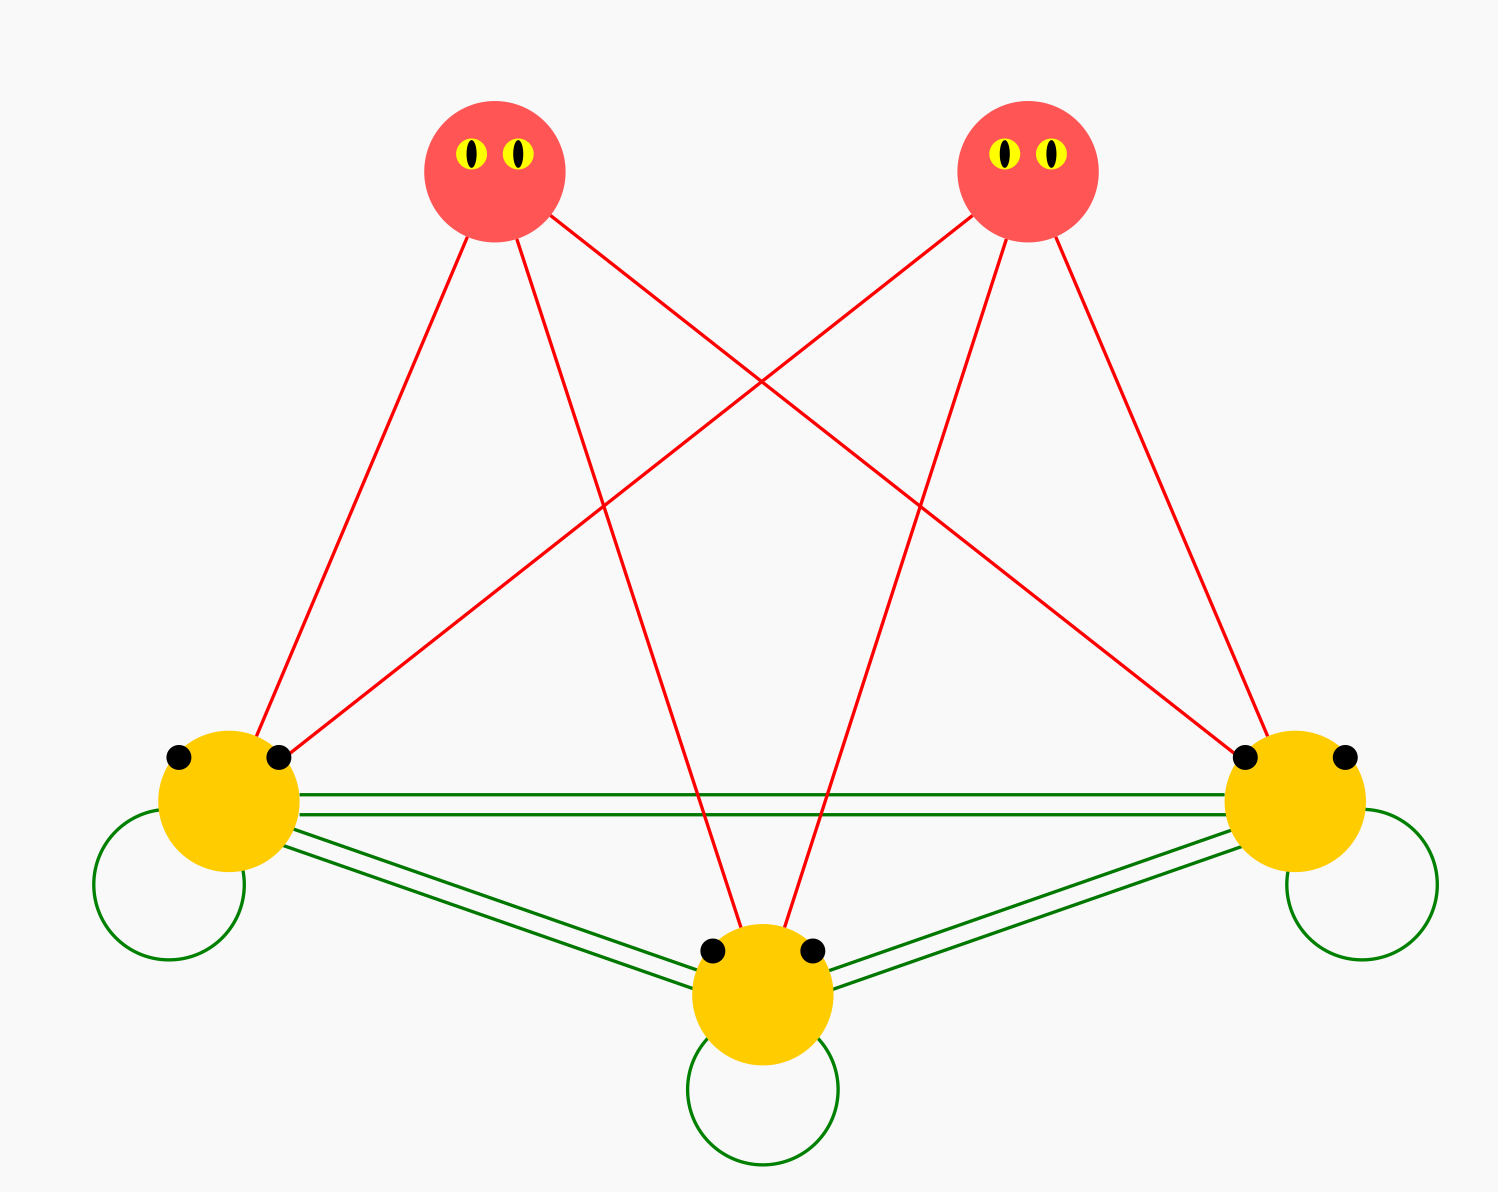
\includegraphics[width=0.7\columnwidth]{net.png}
	\end{center}
	\caption{Example with $2$ consumers and $3$ prey. Each one of the red links represents a predation interaction (coded in the matrix of predator preference coefficients, $ S $). Each green link represents a competition interaction (coded in the matrix of competition coefficients, $ A $). The closed green loops are related with carrying capacity (diagonal elements of $ A $) interpreted here as intra-species competition.}
	\label{fig:Network}
\end{figure}

% Description of the dynamics
The dynamics were modelled as a system of ordinary differential equations. We used the Rosenzweig-MacArthur predator-prey model \cite{Rosenzweig1963} generalized to a higher number of species \cite{Scheffer2004}. Our model is composed of $ n_P $ prey species and $ n_C $ consumer species. $ P_i(t) $ was used for accounting the size of the population of prey $ i $ at time $ t $, and $ C_j(t) $ for the population of consumer $ j $. When it is not explicitly stated, $ i $  runs from $ 1 $ to $ n_P $, and $ j $ from $ 1 $ to $ n_C $. The prey compete directly among themselves, while the consumers compete indirectly by sharing the same food. The consumers eat all kind of prey, but find some of them more preferable than others. All these interactions are summarized in figure \ref{fig:Network}. The overall structure looks like:

\begin{displaymath}
\label{eq:EquationInPseudocode}
	\begin{cases}
	\frac{d}{dt} \left( Prey \right) = Growth  - Predation + Immigration \\
	\frac{d}{dt} \left( Cons \right) = Feeding - Loss \\
	\end{cases}
\end{displaymath}

%% Step-by-step description of each term
The growth term is modelled as a multispecies logistic growth. The strength of the competition between species $ i $ and $ k $ is given by the community matrix element $ A_{ik} $. So, for prey $ i $, we have:

\begin{equation}
\label{eq:Growth-Competition}
%\resizebox{.8 \columnwidth}{!}
%{
Growth_i  = r P_i \left( 1 - \frac{1}{K} \sum_{k=1}^{n_P} A_{ik} \cdot P_k \right)
%}
\end{equation}

A secondary source for prey's growth in our model will be a small constant immigration term $ f $, representing immigration from neighboring areas. Additionally, the inclusion of this term avoids unrealistic long-stretched cycles with near extinctions \cite{Scheffer2004}.

The predator preference for each prey species is given by the matrix $ S $. That is, the matrix element $ S_{ij} $ represents the relative proportion of prey $ i $ in consumer's $ j $ \textit{menu}. We define an auxiliary vector $ V $, whose elements $ V_j $ are calculated as a sum of the prey's populations weighted by the predator preference coefficients. Biologically, this represents the total composition of consumer $ j $'s menu:

\begin{equation}
\label{eq:MenuFunction}
	V_j(P) \equiv \sum_{k=1}^{n_P} S_{jk} \cdot P_k
\end{equation}

We hypothesized that the feeding term will be linear in $ C_j $. The dependency on $V_j$ happens through a Holling type II functional response with half saturation constant $ H $ in order to account for consumer satiation\cite{Edelstein-Keshet}.

\begin{equation}
\label{eq:Feeding}
	Feeding_j = e g C_j \frac{V_j}{V_j+H}
\end{equation}
%TODO Rename feeding
\label{todo:hola}
\todo[inline, color = gray!25, caption = {Rename feeding}]{\textbf{Egbert}: Feeding is confusing as the sum of predation should be the sum of the feeding. Possible new name: GrossGrowth (NetGrowth = GrossGrowth - Loss). \\ \textbf{Pablo}: being the sum up to assimilation constant maybe it is clearer to take the constant out of the equation. \\ \textbf{Pablo}: I'll do it after moving part of this section to the appendix.}

$ e $ represents the assimilation efficiency of the predation. Thus, the effect of consumer $ j $ on all prey's populations is given by $ Feeding_j/e $. Knowing this, we can sum the effect of all consumers in the prey species $ i $ as follows:

\begin{equation}
\label{eq:Predation}
	Predation_i = g \sum_{k=1}^{n_C} \left(\frac{S_{ki}P_i}{V_k}\right) C_k F_{2}(V_j; H)
\end{equation}

Where the term inside the parentheses represents the relative proportion of prey species $ i $ in the menu of predator $ k $, and $F_{2}$ is a shorthand for the Holling type II functional form introduced before. It is interesting to note that the way the predation and feeding terms are defined satisfies the following property:

\begin{equation}
\label{eq:Balance}
	\sum_{j=1}^{n_C} Feeding_j = e \sum_{i=1}^{n_P} Predation_i
\end{equation}

that is, all the deaths at the prey level are invested in the growth of consumers. We define the auxiliary function $ R_i $ as a summary of the effect of all consumers on prey $ i $:

\begin{equation}
\label{eq:PredationAux}
	R_i(P,C) \equiv \sum_{k=1}^{n_C} \left(\frac{S_{ki}P_i}{V_k(P)}\right) C_k F_{2}(V_k(P); H) 
\end{equation}

Putting all together, the dynamical system reads:

\begin{eqnarray}
\label{eq:SystemUnderStudy}
	\begin{cases}
	\dot{P_i} = r P_i \left( 1 - \frac{1}{K} \sum_{k=1}^{n_P} A_{ik} \cdot P_k \right) - g R_i(P,C) + f
	\\ 
	\dot{C_j} = e g C_j F_{2}(V_j(P); H) - l C_j
	\end{cases}
\end{eqnarray}

\begin{figure}
	\begin{center}
		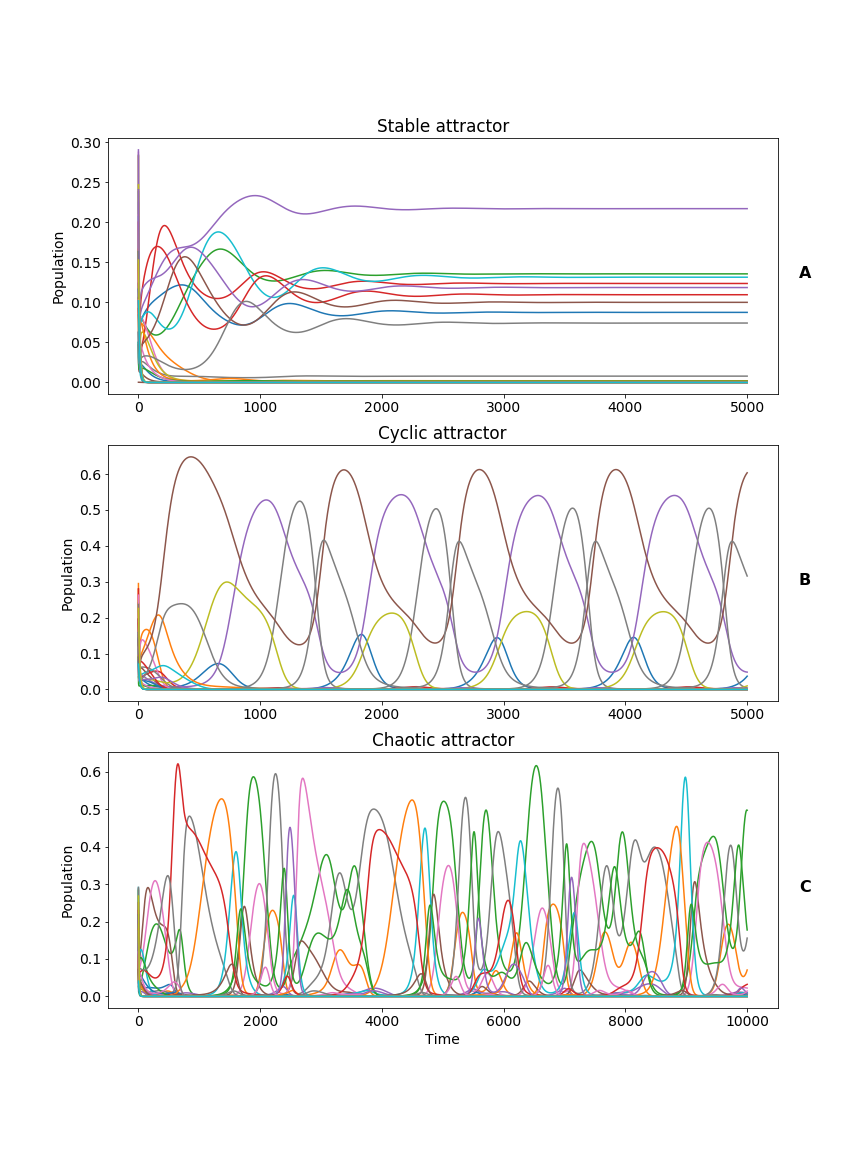
\includegraphics[width=1\columnwidth]{ts.png}
	\end{center}
	\caption{Our model generates time series of the population of each species. The time series can be classified in $3$ qualitative types depending on their asymptotic behavior: \textit{stable}, \textit{periodic} and \textit{chaotic}. In \textbf{figure A}, the system reaches a stable attractor after a transient time. In \textbf{figure B}, a periodic attractor, with an approximate period of 1000 days, is reached after the transient time. The system in \textbf{figure C} never reaches a stable nor a cyclic attractor, but a chaotic one.}
	\label{fig:TimeSeries}
\end{figure}

\subsection{Parameterization}
\label{subsec:Parameterization}
We parameterized our model as a freshwater plankton system based on Dakos' model \cite{Dakos2009b}. Dakos' model, focusing on plankton communities, uses as well a Rosenzweig-McArthur dynamic with two trophic levels (that of zooplankton and phytoplankton). Unlike Dakos, who uses seasonally changing parameters, our parameters were constant (see table \ref{tab:Parameters}).

\begin{table}[H]
	\begin{center}
		\resizebox{\columnwidth}{!}{
		\begin{tabular}{|c|c|c|c|}
			\hline
			\textbf{Symbol} & \textbf{Interpretation} & \textbf{Value} & \textbf{Units} \\
			\hline
			$r$ & Maximum growth rate & $0.50$ & $d^{-1}$ \\
		    \hline
			$K$ & Carrying capacity & $1.00$ & $ mg \ l^{-1} $ \\
			\hline
			$g$ & Predation rate & $0.40$ & $d^{-1}$\\
			\hline
			$f$ & Immigration rate & $10^{-5}$ & $mg \ l^{-1} \ d^{-1}$\\
			\hline
			$e$ & Assimilation efficiency & $0.60$ & $1$\\
			\hline
			$H$ & Half-saturation constant & $2.00$ & $ mg \ l^{-1} $\\
		    \hline
			$l$ & Loss rate & $0.15$ & $d^{-1}$\\
			\hline
		    $S$ & $ n_C \times n_P $ predator preference matrix & $S_{ij} \sim (0,1)$ & $1$\\
		    \hline
   		    $A$ & $ n_P \times n_P $ competition matrix & See section \ref{subsubsec:CompetitionParameter} & $1$\\
		    \hline
		\end{tabular}}
	\end{center}
	\caption{Values and meanings of the parameters used in our numerical experiment}
	\label{tab:Parameters}
\end{table}

\subsubsection{Competition parameter}
\label{subsubsec:CompetitionParameter}

%TODO change parameter name
In order to control how far from neutral the competition is, we introduce the competition parameter $ \epsilon $. This dimensionless parameter allows us to vary continuously from interactions where intraspecific competition is stronger than interspecific (for $ \epsilon < 0 $) to the opposite case (for $ \epsilon > 0$). The border between both cases (i.e. $ \epsilon = 0 $), where neither the intra nor the interspecific competition is dominant, represents neutral competition (see figure \ref{fig:CompetitionParameter} in Appendix).

The numerical implementation of these ideas can be easily achieved by building a competition matrix whose diagonal terms are identically $ 1 $, and whose non-diagonal terms are drawn from a uniform probability distribution centered at $ 1 + \epsilon $ and with a given width (here we chose $ w = 0.2$).

This parameterization allows us to travel continuously from strong dominant intraspecific ($ \epsilon < 0$) to strong interspecific competition ($ \epsilon > 0$), meeting neutral competition at the border in between (i.e., at $\epsilon = 0$).

\subsection{Numerical experiment}
\label{subsec:NumericalExperiment}
Depending on the parameters and the initial conditions, the system described in equation \ref{eq:SystemUnderStudy} can give rise to three types of asymptotic behavior, each of them roughly corresponding to a different type of attractor (see figure \ref{fig:TimeSeries}). The easier one, corresponding to a stable point attractor, generates a constant species composition. Limit cycle (and limit tori) attractors give rise to periodically (or quasiperiodically) changing species composition. Last but not least, we'll refer as chaotic to attractors not fitting in any of the previous categories.

Our target is to estimate the probability of reaching one of such chaotic attractors under different assumptions about intraspecific competition. In order to achieve this, we simulated several ecosystems with different initial conditions and relative predation intensities, but sharing the same competition parameter.

Numerical methods are used to integrate the equation \ref{eq:SystemUnderStudy}. A first stabilizing run of $ 2000 $ days is generated in order to get closer to the attractor. Simulating for $ 5000 $ more days, we obtain time series as the ones in figure \ref{fig:TimeSeries}. 

In the exploratory phase of this research three parallel approaches to chaos detection were followed: Lyapunov exponents estimation \cite{Strogatz1994}, Gottwald-Melbourne \textit{0-1} test \cite{Gottwald2009} and visual inspection. Despite differences in the exact probabilities, the three of them led us to the same qualitative conclusions. We found the results of the Gottwald-Melbourne test most consistent with visual inspection. We called chaotic all those time series complicated enough to trigger the Gottwald-Melbourne test. Using this approach, we classified each individual simulation as \textit{chaotic} or \textit{non-chaotic}. Our numerical experiment was repeated $ 200 $ times for each competition parameter. The ratio of attractors found to be chaotic can be used to estimate the probability of ecosystems of a given degree of heterogeneity developing chaotic asymptotic behavior.

Additionally, the experiment was repeated for food webs of different sizes. In our simulations, we kept a ratio of 2:3 for the number of species at the consumer and the prey level.

For the sake of reproducibility, we provide a \textit{GitHub} link to the analysis scripts used\footnote{https://github.com/PabRod/Chaos-and-neutrality}. For further information, please refer to the \textit{read me} file and/or to the Appendix.

\section{Results}
\label{sec:Results}
Plotting the probability of chaos against the competition parameter (see figures \ref{fig:Results}), we observe a clear maximum around $ \epsilon = 0 $. That is, for neutral competition at the prey's trophic level, the likelihood of chaotic behaviour is higher than for dominant inter or intraspecific competition. This result remains true for systems with different amount of species (figures \ref{fig:Results} and \ref{fig:Contour}).

The overall likelihood of chaos, which can be interpreted as the area under the curve in figure \ref{fig:Results}, increases with the size of the food web. This effect should not be surprising: the more dimensions the phase space has, the easier is to fulfill the requirements of the complex geometry of a chaotic attractor \cite{Strogatz1994}. We can understand this intuitively as increasing the available room for the trajectories to pack closer and closer without ever crossing each other nor collapsing to a point. Even in those higher dimensional cases, there is still a clear maximum at neutral competition.

% Weak and strong interspecific competition
There's another local maximum for $ \epsilon = -1 $. This means that weak competition coupling, in our model, also promotes chaos.

Between both local maxima there is obviously a local minimum whose exact position differed between experiments.

\begin{figure}
	\begin{center}
		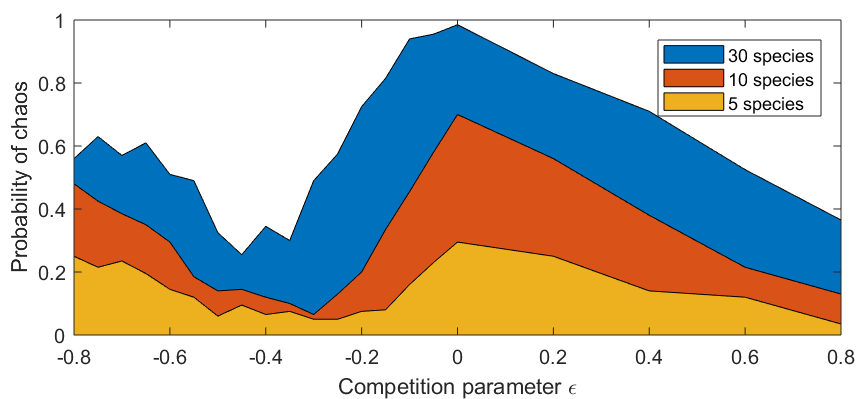
\includegraphics[width=1\columnwidth]{results.png}
	\end{center}
	\caption{Results for a low, medium and high dimensional system. Notice how the probability of chaos has a local maximum around $\epsilon = 0$. The overall probability of chaos, understood as the area under the curve, grows with the system size. The local maximum stays at $\epsilon = 0$ even for systems with a big amount of species.}
	\label{fig:Results}
\end{figure}

\begin{figure}
	\begin{center}
		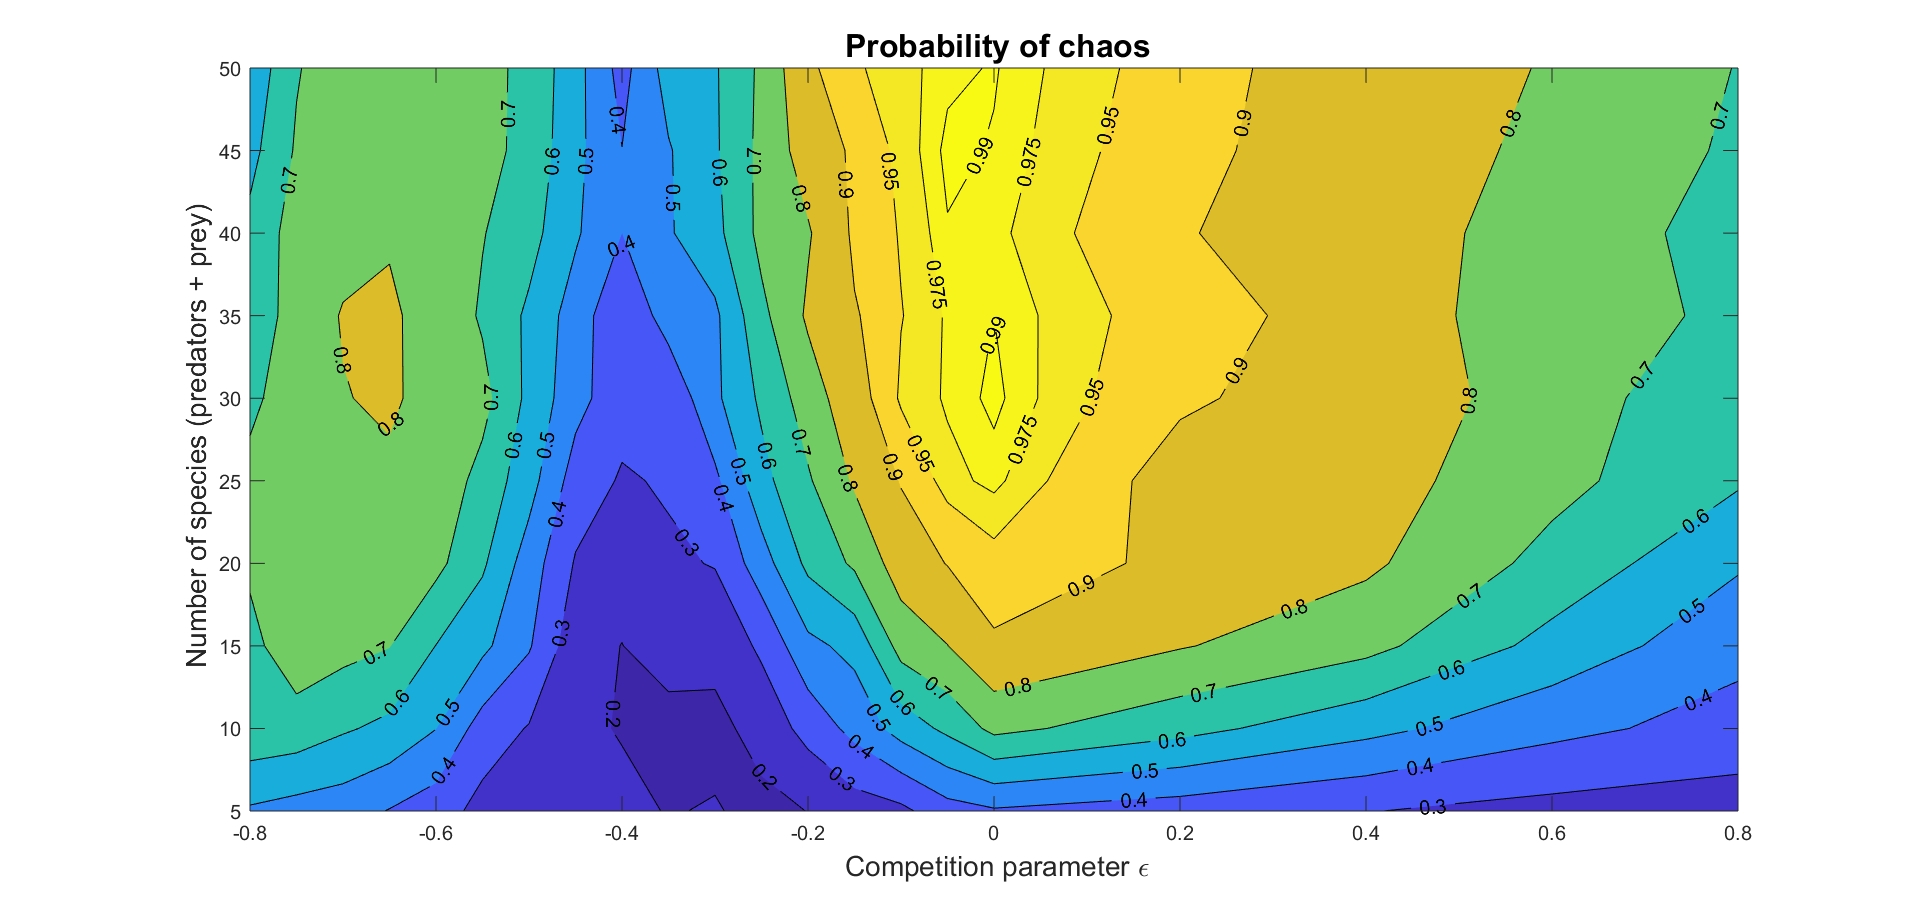
\includegraphics[width=1\columnwidth]{contour.png}
	\end{center}
	\caption{Contour map showing the probability of chaos for various competition parameters (horizontal axis) and number of species (vertical axis). The consumers' population is fixed as $ 2/3 $ of the prey's population. Notice that chaotic attractors appear more easily (i.e., for smaller systems) the closer is the competition to neutral (i.e., $ \epsilon = 0 $).}
	\label{fig:Contour}
\end{figure}

\section{Discussion}
\label{sec:Discussion}
% Our claims
The asymptotic dynamics of our model are affected by how strong intraspecific competition compared to interspecific competition is. We find particularly interesting the fact that the closer to neutrality the competition in our food web is, the higher are the chances of developing chaotic behaviour. This suggests that in a system with predation, near-neutrality at the competition level may increase the probability of complex dynamics if the species are not equally prone to predation. Provided the competitive exclusion principle rests on the assumption of equilibrium, near-neutrality reduces the chances of the principle to be applicable, improving the chance for a higher number of coexisting species. Additionaly, this observation suggests that the hypothesis of non-equilibrium and Hubbell's hypothesis of neutrality are not completely independent. Our model shows another local maximum for the probability of chaos for weak competition coupling. We consider this a reasonable result, as predation is known to be the main driver of chaos in this kind of models \cite{Scheffer2004}.

%% Limitations
% Why two levels?
In the spirit of mathematical modelling, we chose the simplest realization required for the effects to be observed. We didn't use Allee effect, nor noise, and the functional form of each term has been chosen to account for satiation and saturation in the simplest possible ways. The choice of a two-level model may seem in contradiction with the pursue of simplicity, but actually it is a fundamental requirement for the effect under research to take place. In the absence of a predator level, chaos will never develop in a model with neutral competition. The reason for this is that if all interactions become equally strong, the differences among species at the same trophic level fade out. This makes labeling each species meaningless, and thus the prey-only system can be reduced just to one differential equation, that of the total population (see section \ref{subsec:NeutralCompetition} for details). Using the Poincar�-Bendixson theorem, it can be proven that chaos autonomous systems with less than $3$ dimensions cannot exhibit chaos \cite{Strogatz1994}. 

Even in the absence of neutral competition, it is known that the presence of chaos or cycles instead of fixed points depends crucially on predation and its heterogeneity \cite{Scheffer2004}. This predation effects can be interpreted as a type of response diversity \cite{Yachi1999}, so including them provides additional realism to the model.

% Choice of interaction parameters: modularity
Both the competition and predation parameters were drawn from probability distributions. The interactions in our system can be interpreted as a weighted network with a high connectivity. Trophic networks studied in nature tend to show modular structure with various clusters \cite{Thebault2010}. The present model restricts its attention on one of those modules, neglecting possible interactions with others.

% Choice of interaction parameters: randomness
It is known that the asymptotic behaviour of this kind of systems can be very sensitive to the parameters choice. In particular, introducing correlations between parameters can greatly modify the probabilities of chaotic attractors to be reached (see for instance \cite{Huisman2001}, in response to the letter \cite{Schippers2001}). In the present paper we didn't introduce any correlation, i.e., all our random parameters were drawn independently from the others. Studying the effect of different physiological scenarios (in the sense of \cite{Huisman2001}, that is, constrains between the parameters) on the probabilities of chaos could be a continuation to this paper.

% Role of symmetry
%TODO Effects of symmetry, show or not mention
%It may be worth noting that the position of both the maxima we've found (i.e.: $ \epsilon = -1 $ and $ \epsilon = 0 $) have something in common: the community matrix $ A $ at those values of the parameter is very symmetric in both cases. It will be interesting to develop a similar method that, instead of varying neutrality, varies the less restrictive property of symmetry.
%\todo[inline, color=blue!25, caption={Effects of symmetry}]{\textbf{Egbert}: Good chance that a reviewer says: nice these suggestions, but why do they not show it here? \\ \textbf{Pablo}: Remove or do? \\ \textbf{Egbert}: up to you. Maybe it is not so difficult to perform the same analysis imposing symmetry}

% Chaos detection
Due to the large amount of simulations made, we had to rely in automatic methods for detecting chaos. Numerical detection of chaos has fundamental limitations. All of them can be boiled down to the fact that, in general, numerical methods cannot distinguish robustly between long, complicated transients and genuine chaos. We think that our approach to chaos detection, despite being open to improvement, suffices to hold the biological conclusions.

% Concluding remark
The paradox of biodiversity is a tremendously complex scientific problem. With these model exercises we definitely do not claim to have solved it, but we show that predation in combination with neutral competition may increase the probability of chaos, and thereby increase the number of coexisting species.

% Is chaos more resilient?
%Additionally, we are implicitly assuming without a proof that chaotic ecosystems can have more species %than non-chaotic ones\todo{Stronger concluding remark required}.
%\todo[inline, caption={This is well known in math}]{There are mathematical reasons for this to be true. Keywords: uniformly hyperbolic dynamical systems, Anosov maps, Arnold's cat map.}
%%TODO there are mathematical reasons for this to be true. Keywords: uniformly hyperbolic dynamical systems, Anosov maps, Arnond's cat map

%%TODO A possible continuation of this research may be the setting of two indepedent ecosystems, one of them chaotic and the other one non-chaotic, and allow them to interact at some point of time (simulating an invasion), in order to assess how much of each of the original ecosystems survives to this traumatic event. This is a good idea, but I think testing for resilience is too far from this study to put it here. You could instead refer to the discussions about  Huismans paper (Schippers, P., A. M. Verschoor, M. Vos, and W. M. Mooij. 2001. Does "supersaturated coexistence" resolve the "paradox of the plankton"? Ecology letters 4:404-407. and Huismans reply) {Schippers2001}

\section{Acknowledgements}
\label{sec:Acknowledgements}
The preliminary analysis of this model were performed using GRIND for Matlab (http://www.sparcs-center.org/grind). Additionally, we thank prof. Sebastian Wieczorek, Jelle Lever, Moussa N'Dour and Sebastian Bathiany for their useful comments and suggestions.

\clearpage

\section{Appendix}
\label{sec:Appendix}

\subsection{Generalized multispecies predation models}
\label{subsec:GeneralizedModels}

\subsubsection{General properties of predation models}
\label{subsubsec:GeneralPropertiesOfPredation}

Most predation models based on differential equations follow a structure like this:

\begin{eqnarray}
\label{eq:CommonStructure}
	\begin{cases}
	\dot{P} = Growth(P) - Predation(P,C)
	\\ 
	\dot{C} = -Loss(C) + GrossGrowth(P,C)
	\end{cases}
\end{eqnarray}

where $P$ represents the biomass of the prey population, and $C$ the biomass of the consumer/predator population. The functional dependences have been explicitly written in order to remark the fact that the coupling of the system happens via the $Predation$ and $GrossGrowth$ terms.

It is important to note that, in models like this, all deaths at the prey's level are due to predation. This can be understood as all deaths being \textit{invested} into consumer's growth. In order of this effect to be true, a restriction must be applied to the functional forms of $Predation$ and $CrossGrowth$:

\begin{equation}
\label{eq:InnerEnergyFlow}
	GrossGrowth(P,C) = e \cdot Predation(P,C)
\end{equation}

where $e$ represents the efficiency of the energy transfer process. Equation \ref{eq:InnerEnergyFlow}, when plugged into \ref{eq:CommonStructure}, yields:

\begin{equation}
\label{eq:AllEnergyFlow}
	e \dot P + \dot C = e \cdot Growth(P) - Loss(C)
\end{equation}

Equation \ref{eq:AllEnergyFlow} allows us to think of our system as an open system from the point of view of thermodynamics, with $Growth$ being the only source of the system, and $Loss$ the only sink (see figure \ref{fig:EnergyFlow}). All the energy exchange due to predation stays inside the system, so predation can be considered a closed subsystem.

\begin{figure}
	\begin{center}
		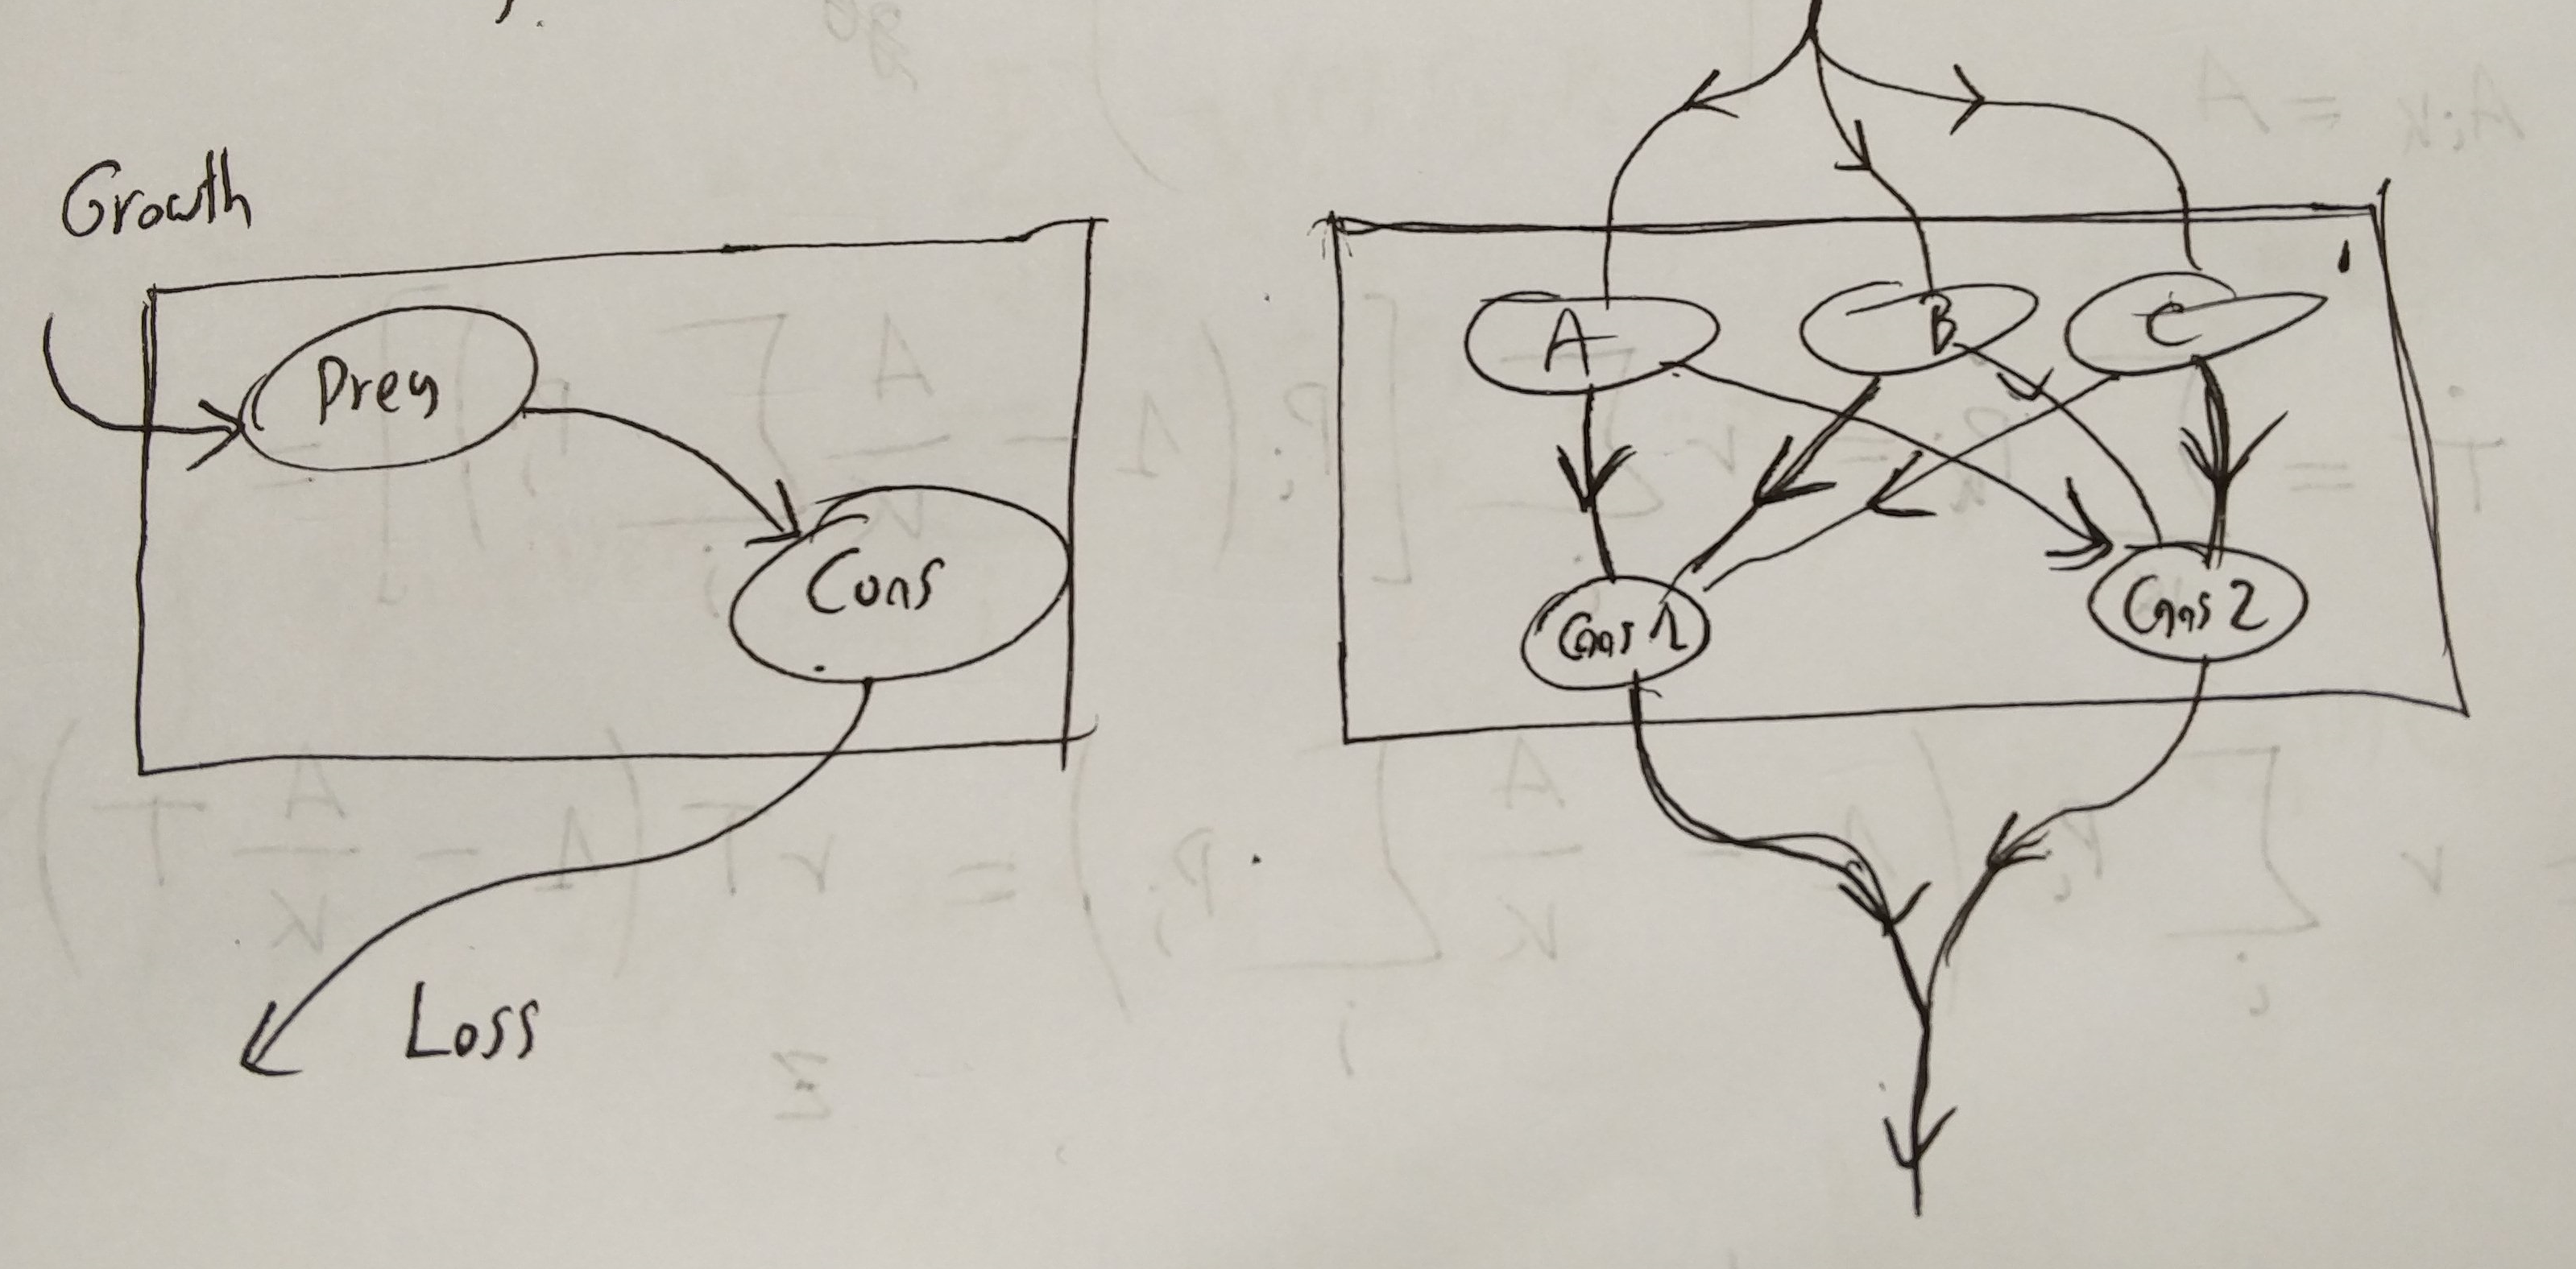
\includegraphics[width=1\columnwidth]{energyflow.png}
	\end{center}
	\caption{Plot showing the energy flow for a two species and a multispecies system.}
	\label{fig:EnergyFlow}
\end{figure}

We can generalize this basic structure to multispecies, two trophic levels systems. First, we'll go back to equation \ref{eq:CommonStructure} and just add more rows, being specially careful with the variables inside the functional relations:

\begin{eqnarray}
\label{eq:CommonStructureMulti}
	\begin{cases}
	\dot{P_i} = Growth_i(P) - Predation_i(P,C) & : i = 1..n_P
	\\ 
	\dot{C_j} = -Loss_j(C_j) + GrossGrowth_j(P,C_j) & : j = 1..n_C
	\end{cases}
\end{eqnarray}

where now $i$ runs from $1$ to the number of prey $n_P$ and $j$ from $1$ to the number of consumers $n_C$. Here, we've used $P_i$ to denote the population of the prey labeled by $i$, and $P$ for the vector containing all prey populations. Notice that, while the $Growth$ term can involve competition (and thus, depends on the whole vector $P$), the $Loss$ term for species $j$ depends only in the population of that species (i.e.: $C_j$), regardless of the rest.

Requiring once again our predation to be fully invested in consumer's growth, we find the following generalization of equation \ref{eq:InnerEnergyFlow}:

\begin{equation}
\label{eq:InnerEnergyFlowMulti}
	\sum_{j = 1}^{n_C} GrossGrowth_j(P,C_j) = \sum_{i = 1}^{n_P} e_i \cdot Predation_i(P,C)
\end{equation}

Using \ref{eq:InnerEnergyFlowMulti} and \ref{eq:CommonStructureMulti}, it is easy to prove that the multispecies generalization of \ref{eq:AllEnergyFlow} is:

\begin{equation}
\label{eq:AllEnergyFlowMulti}
	\sum_{i = 1}^{n_P} e_i \dot P_i + \sum_{j = 1}^{n_C} \dot C_j = \sum_{i = 1}^{n_P} e_i \cdot Growth_i(P) - \sum_{j = 1}^{n_C} Loss_j(C_j)
\end{equation}

The intuitive interpretation is, again, that the sinks and sources of energy in our systems are the total $Loss$ and $Growth$.

It is difficult to overestimate the importance of restriction \ref{eq:InnerEnergyFlowMulti} (or equivalently, \ref{eq:AllEnergyFlowMulti}). We need it to build realistic functional forms for the coupling terms. Being the coupled terms those related with predation, those terms are the very core of this models.

\subsubsection{Lotka-Volterra equations}
\label{subsubsec:LotkaVolterra}
The most basic model of predation is the Lotka-Volterra system of equations:

\begin{eqnarray}
\label{eq:LotkaVolterra}
	\begin{cases}
	\dot{P} = r P - g P C
	\\ 
	\dot{C} = - l C + e g C P
	\end{cases}
\end{eqnarray}

Where $r$ represents the growth rate of the prey, $g$ the grazing rate of the predator against the prey, $l$ the loss rate of the predator and $e$ the efficiency conversion factor.

It is trivial to prove that the Lotka-Volterra model satisfies the requirements shown in subsection \ref{subsubsec:GeneralPropertiesOfPredation}. 

\subsubsection{Multispecies Lotka-Volterra equations}
\label{subsubsec:LotkaVolterraMulti}

Lotka-Volterra equations can be generalized to a model with multiple species by noting that each prey will be affected by all consumers, and each consumer will be affected by all prey. In order to code the strength of this interactions, we introduce the matrix $S$, whose element $S_{ji}$ gives the strength of the coupling of consumer $j$ and prey $i$. As a consequence: for prey dynamics, this matrix is scanned row-wise, while for predators it is scanned column-wise. The generalized system looks like:

\begin{eqnarray}
\label{eq:LotkaVolterraMulti}
	\begin{cases}
	\dot{P_i} = r_i P_i - P_i \sum_{j = 1}^{n_C} g_j S_{ji} C_j & : i = 1..n_P
	\\ 
	\dot{C_j} = - l_j C_j +  g_j e_j C_j \sum_{i = 1}^{n_P} S_{ji} P_i  & : j = 1..n_C
	\end{cases}
\end{eqnarray}

The fulfillment of condition \ref{eq:InnerEnergyFlowMulti} is again easily proven.

In this model, all terms can grow without boundaries. This is not only unrealistic, but also creates some problems from the sole point of view of mathematical stability.

\subsubsection{Rosenzweig-MacArthur model}
\label{subsubsec:Rosenzweig-MacArthur}
The Rosenzweig-MacArthur predator-prey model improves the previous model by adding boundaries to the terms' dependency on the prey population. This is achieved by encapsulating $P$ inside saturating functions. In particular, the growth rate $r$ now depends on $P$, and the grazing rate $g$ in the coupling terms is now a function of $P$ (see equation \ref{eq:RosMac2levels} and compare it with \ref{eq:LotkaVolterra}).

\begin{eqnarray}
\label{eq:RosMac2levels}
	\begin{cases}
	\dot{P} = r(P) P - g(P) P C
	\\ 
	\dot{C} = - l C + e g(P) C P
	\end{cases}
\end{eqnarray}

Once again, condition \ref{eq:InnerEnergyFlow} is trivially fulfilled independently of the functional form of $r(P)$ and $g(P)$. If those both functions are chosen appropriately, we avoid unbounded effects. Typically a logistic growth form is chosen for $r(P)$, that is, $r(P) = r_0 \left(1 - \frac{P}{K} \right)$, and a Holling type II functional form for the grazing $g(P)$, that is, $g(P) = \frac{g_0}{P+H}$. After making this choices, our system takes its classical form:

\begin{eqnarray}
\label{eq:RosMac2classic}
	\begin{cases}
	\dot{P} =  r P \left( 1 - \frac{P}{K} \right) - g C \frac{P}{P + H}
	\\ 
	\dot{C} = - l C + e g C \frac{P}{P + H}
	\end{cases}
\end{eqnarray}

\subsubsection{Multispecies Rosenzweig-MacArthur model}
\label{subsubsec:Rosenzweig-MacArthurMulti}

Noticing the similarities between equations \ref{eq:LotkaVolterra} and \ref{eq:RosMac2levels}, the latter can be generalized in the same fashion as we did to obtain \ref{eq:LotkaVolterraMulti}, yielding:

\begin{eqnarray}
\label{eq:RosMacMulti}
	\begin{cases}
	\dot{P_i} = r_i(P) P_i - P_i \sum_{j = 1}^{n_C} g_j(P) S_{ji} C_j & : i = 1..n_P
	\\ 
	\dot{C_j} = - l_j C_j +  g_j(P) e_j C_j \sum_{i = 1}^{n_P} S_{ji} P_i  & : j = 1..n_C
	\end{cases}
\end{eqnarray}

Written like this, it is easy to see that the condition \ref{eq:InnerEnergyFlowMulti} is fulfilled. 

Regarding the proper functional forms of $r_i(P)$ and $g_j(P)$, our growth term has to take into account both the inter and intraspecific competition. This can be easily modelled by choosing:

\begin{equation}
\label{eq:r}
	r_i(P) = r_i \left( 1 - \sum_{k=1}^{n_P} A_{ik} P_k \right)
\end{equation}

We hypothesize that the grazing rates corresponding to predator $j$, that is, $g_j(P)$, follow a Holling type II functional response dependent on the total consumption of prey by predator $j$, that is: $V_j(P) \equiv \sum_{i=1}^{n_P} S_{ji} P_i$

\begin{eqnarray}
\label{eq:g}
	g_j(P) = \frac{g_j}{V_j + H_j} = \frac{g_j}{\sum_{i=1}^{n_P} S_{ji} P_i + H_j}
\end{eqnarray}

\subsubsection{Summary}
\label{subsubsec:SummaryPredation}

\begin{table}[H]
\label{tab:SummaryPredation}
	\begin{center}
		\resizebox{\columnwidth}{!}{
			\begin{tabular}{|c|c|c|} \hline 
				 & Two species & Multispecies \\ 
				\hline 
				Lotka-Volterra & $\begin{cases}\dot{P} = r P - g P C\\ \dot{C} = - l C + e g C P\end{cases}$ & $\begin{cases} \dot{P_i} = r_i P_i - P_i \sum_{j = 1}^{n_C} g_j S_{ji} C_j \\ \dot{C_j} = - l_j C_j +  g_j e_j C_j \sum_{i = 1}^{n_P} S_{ji} P_i \end{cases}$ \\ 
				\hline 
				Rosenzweig-MacArthur & $\begin{cases}\dot{P} = r(P) P - g(P) P C\\\dot{C} = - l C + e g(P) C P\end{cases}$ & $\begin{cases} \dot{P_i} = r_i(P) P_i - P_i \sum_{j = 1}^{n_C} g_j(P) S_{ji} C_j \\ \dot{C_j} = - l_j C_j +  g_j(P) e_j C_j \sum_{i = 1}^{n_P} S_{ji} P_i \end{cases}$  \\
			\hline  \end{tabular}}
	\end{center}
	\caption{Summary table with the different types of predation models studied. Written this way, the parallelisms are obvious. In multispecies models, the index $i$ runs from $1$ to $n_P$, and $j$ from $1$ to $n_C$. The functional forms of $r_i(P)$ and $g_j(P)$ are given in equations \ref{eq:r} and \ref{eq:g}}
\end{table}

\subsection{Neutral competition and system degeneration}
\label{subsec:NeutralCompetition}
%TODO Check name
\todo[inline, color = gray!25, caption = {Check name}]{\textbf{Pablo}: Check degeneration is the correct word}
If we drop everything but the competition part of our dynamics (see equation \ref{eq:SystemUnderStudy}), we will find a system of $ n_P $ equations like the following:

\begin{eqnarray}
\label{eq:OnlyCompetition}
\dot{P_i} = r P_i \left( 1 - \frac{1}{K} \sum_{k=1}^{n_P} A_{ik} \cdot P_k \right)
\end{eqnarray}

In order to model a neutral competition, we should use the same competition coefficient for each interaction between species. That is, take $ A_{ik} = A $ for all $ i $ and $ k $. Equation \ref{eq:OnlyCompetition} then becomes:

\begin{eqnarray}
\label{eq:OnlyNeutralCompetition}
\dot{P_i} = r P_i \left( 1 - \frac{A}{K} \sum_{k=1}^{n_P} P_k \right)
\end{eqnarray}

From equation \ref{eq:OnlyNeutralCompetition} we see that all species have exactly the same dynamical equation. This will make the nullclines to coincide at all points, so the equilibrium points will degenerate to equilibrium manifolds (see figure \ref{fig:Neutral}).

\begin{figure}[h]
	\begin{center}
		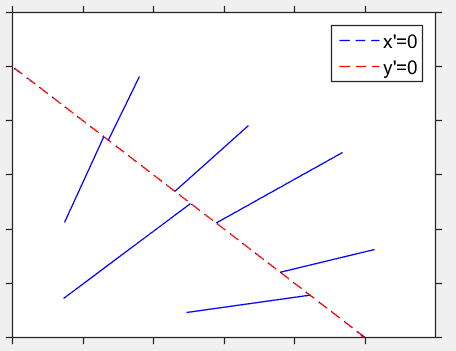
\includegraphics[width=0.9\columnwidth]{degenerate.png}
	\end{center}
	\caption{Example with $2$ prey under neutral competition. Both nullclines coincide point to point, giving rise to a higher dimensional equilibirium manifold (in this case, a straight line)}
	\label{fig:Neutral}
\end{figure}

This problem can be solved noticing that, in a competition-only system, the effect of neutrality is to fade out the differences between species. Being this the case, the labels $ i $ distinguishing them become meaningless. It is a natural idea to sum up all the biomasses of competing species into a new variable, that of total population of (now indistinguishable) species, defined by:

\begin{eqnarray}
\label{eq:TotalPopulation}
	T(t) = \sum_{i=1}^{n_P} P_i(t)
\end{eqnarray}

In agreement with the biological intuition, manipulating \ref{eq:TotalPopulation} and \ref{eq:OnlyNeutralCompetition} it can be proved (see eq. \ref{eq:TotalPopulationDynamics}), that the total population biomass will follow the same differential equation as the individual species abundances (i.e., equation \ref{eq:OnlyNeutralCompetition}). 

\begin{eqnarray}
\label{eq:TotalPopulationDynamics}
	\dot T = \sum_{i=1}^{n_P} \dot P_i = r \sum_{i=1}^{n_P} P_i \left( 1 - \frac{A}{K} \sum_{k=1}^{n_P} P_k \right) = r T (1 - \frac{A}{K} T)
\end{eqnarray}

Additionally, this result shows that we are actually working with a one-dimensional system, being the apparent $ n_P $ dimensions of our original problem an artifact due to a wrong choice of state variables. In our model, the predation interaction breaks this excess of symmetry, so we can still work with neutral competition as long as the predation is not neutral without facing problems of system degeneration.


\subsection{Extra figures}
\label{subsec:ExtraFigures}

\subsubsection{Competition matrix}
\label{subsubsec:CompetitionMatrix}

\begin{figure}[H]
	\begin{center}
		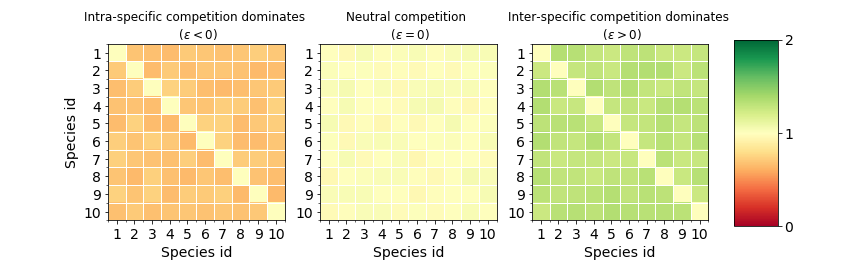
\includegraphics[width=1\columnwidth]{epsilon_all.png}
	\end{center}
	\caption{The competition matrix on the left is a clear case of dominant intraspecific competition. The central one represents a case of neutral competition. The matrix in the right panel shows a case of dominant interspecific competition. The difference between them is the relative size of the non-diagonal elements respective of the diagonal ones. This qualitative property of the competition matrices is controlled by the parameter $\epsilon$.}	
	\label{fig:CompetitionParameter}
\end{figure}

\subsubsection{Flow chart}
\label{subsubsec:FlowChart}

\begin{figure}[H]
	\begin{center}
		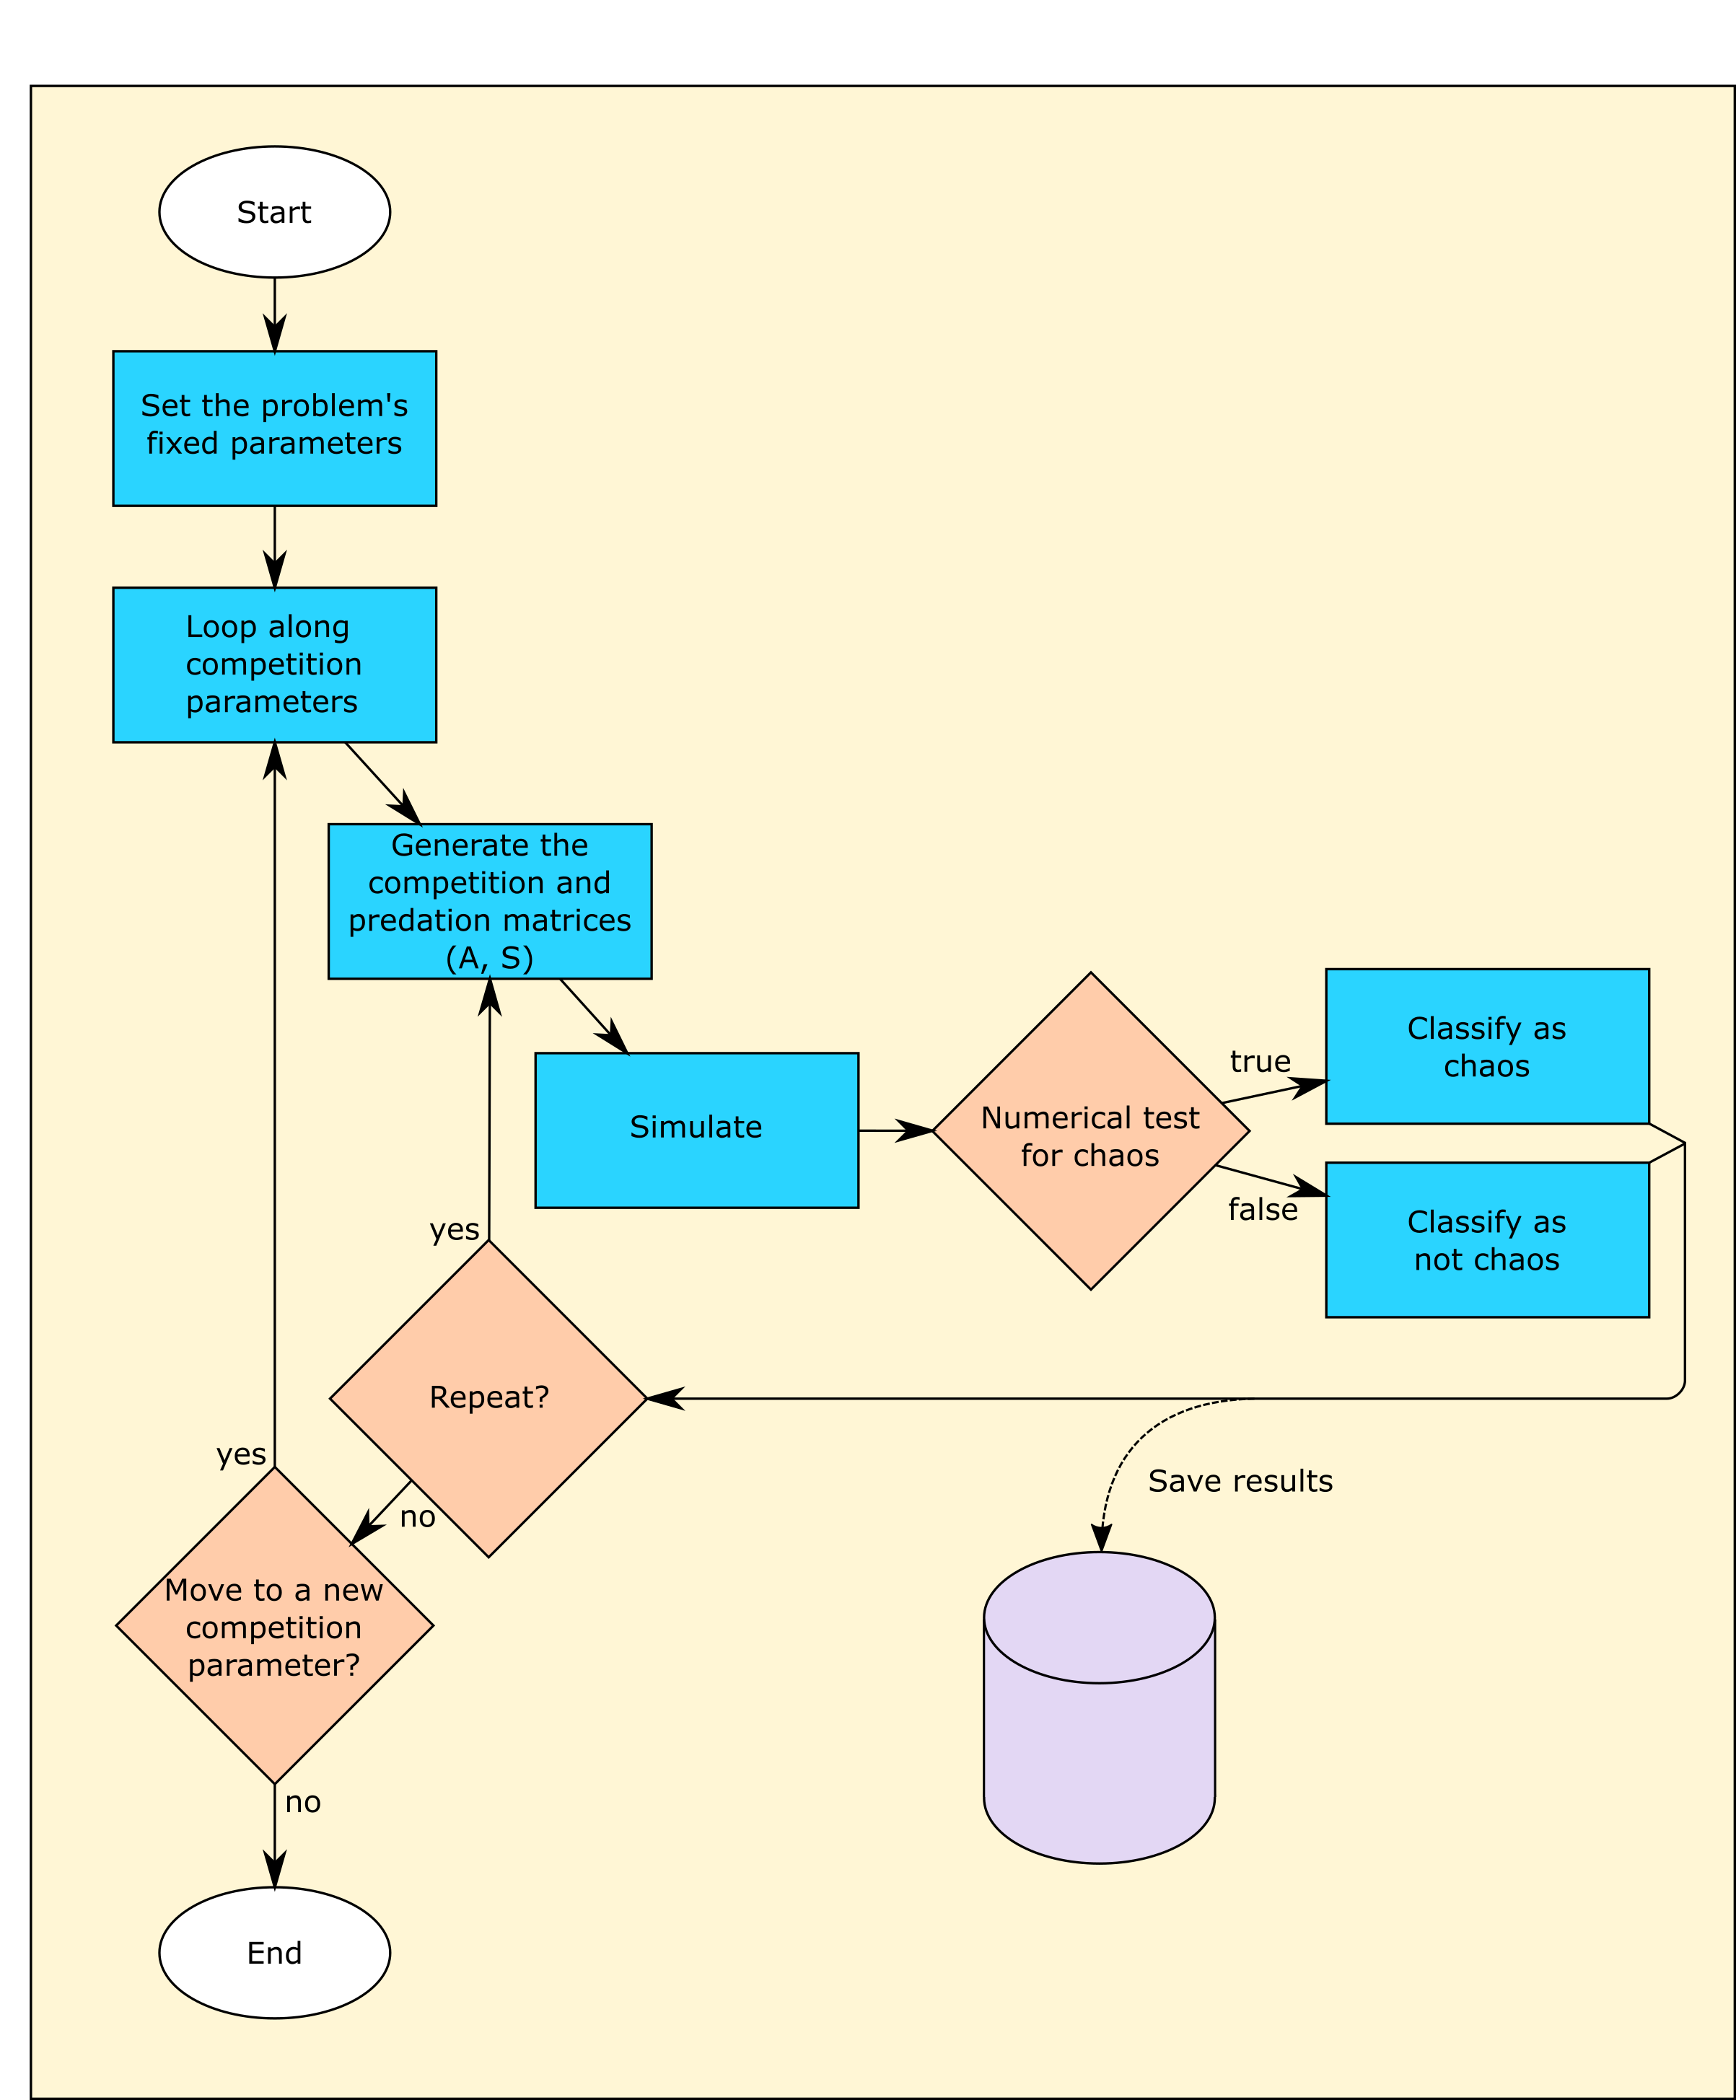
\includegraphics[width=0.9\columnwidth]{flow_chart.png}
	\end{center}
	\caption{Flow chart describing the numerical experiment. The source code is available at \textit{https://github.com/PabRod/Chaos-and-neutrality}.}
	\label{fig:FlowChart}
\end{figure}

%
%\subsection{Detection of chaos}
%\label{subsec:DetectionOfChaos}
%Dynamical systems with chaotic attractors are extremely sensitive to initial conditions. Two trajectories whose initial conditions are slightly different will diverge exponentially if they lie in the basin of a chaotic attractor. The initial rate of divergence is quantified by the Lyapunov exponent \cite{Strogatz1994}.
%
%Our procedure for classifying the attractors as chaotic or non-chaotic was based in the analysis of Lyapunov exponents. More specifically, this is the procedure we've followed:
%
%\begin{enumerate}
%	\item \label{GoToAttractor} Run the simulation for a sufficient time, in order to guarantee that a trajectory reached an attractor and the dynamics are asymptotic.
%	\item \label{RunInAttractor} Use the last point of the run in step \ref{GoToAttractor} as a starting point for a second, shorter run on the attractor.
%	\item \label{PerturbedTrajectory} Use again the last point of the run in step \ref{GoToAttractor} but, this time, adding a small disturbance to it.
%	\item Compare the runs in steps \ref{RunInAttractor} and \ref{PerturbedTrajectory} to compute numerically the principal Lyapunov exponent.
%	\begin{itemize}
%		\item If it's positive, classify the attractor as chaotic.
%		\item If it's negative, classify the attractor as non-chaotic.
%	\end{itemize}
%\end{enumerate}

\clearpage

\bibliography{library}
\bibliographystyle{vancouver}

%\listoftables
%\listoffigures

%TODO Create an online appendix with extra figures, different chaos tests, different random distributions
\todo[inline, color = gray!25, caption={Online appendix}]{Decide how to split the information into main paper + appendix. \textbf{Egbert}: I think you need to make an appendix explaining the relation between Lyapunov and the other indices. Maybe some additional figures (if you have them?) In the results section you should refer to those extra results. }
%TODO Past tense
\todo[inline, color = gray!25, caption={Past tense}]{Double check the use of past tense along all the paper}

\end{document}